
% debut d'un fichier latex standard
\documentclass[a4paper,12pt,twoside]{article}

% pour l'inclusion de figures en eps,pdf,jpg
\usepackage{graphicx}
\usepackage{subcaption}
\usepackage{wrapfig}
\usepackage{siunitx} % pour utiliser les unités SI. Commande à utiliser: \SI{quantité}{unité}
% quelques symboles mathematiques en plus
\usepackage{amsmath}
% le tout en langue francaise
\usepackage[french]{babel}
% on peut ecrire directement les caracteres avec l'accent
% a utiliser sur Linux/Windows
\usepackage[utf8]{inputenc}
\usepackage[T1]{fontenc}
% a utiliser sur le Mac
%\usepackage[applemac]{inputenc}
% pour l'inclusion de links dans le document 
\usepackage[colorlinks,bookmarks=false,linkcolor=blue,urlcolor=blue]{hyperref}

\paperheight=297mm
\paperwidth=210mm

\setlength{\textheight}{235mm}
\setlength{\topmargin}{-1.2cm} % pour centrer la page verticalement
%\setlength{\footskip}{5mm}
\setlength{\textwidth}{15cm}
\setlength{\oddsidemargin}{0.56cm}
\setlength{\evensidemargin}{0.56cm}

\pagestyle{plain}

% quelques abreviations utiles
\def \be {\begin{equation}}
\def \ee {\end{equation}}
\def \dd  {{\rm d}}

\newcommand{\mail}[1]{{\href{mailto:#1}{#1}}}
\newcommand{\ftplink}[1]{{\href{ftp://#1}{#1}}}
%
% latex SqueletteRapport.tex      % compile la source LaTeX
% xdvi SqueletteRapport.dvi &     % visualise le resultat
% dvips -t a4 -o SqueletteRapport.ps SqueletteRapport % produit un PostScript
% ps2pdf SqueletteRapport.ps      % convertit en pdf

% pdflatex SqueletteRapport.pdf    % compile et produit un pdf

% ======= Le document commence ici ======

\begin{document}
% Le titre, l'auteur et la date
\title{De la Terre à la Lune\\{\small Physique Numérique I}\\{\small Rapport 1}}
\date{\today}
\author{Delphine Martres et Damien Korber\\{\small \mail{delphine.martres@epfl.ch} et \mail{damien.korber@epfl.ch}}}
\maketitle
\tableofcontents % Table des matieres

% Quelques options pour les espacements entre lignes, l'identation 
% des nouveaux paragraphes, et l'espacement entre paragraphes
\baselineskip=16pt
\parindent=15pt
\parskip=5pt



%%%% ON COMMENCE A ECRIRE D'ICI

\section{Introduction}
Le roman de Jules Vernes \textit{"De la Terre à la Lune"} décrit une méthode originale pour envoyer des projectiles jusqu'à la Lune à l'aide d'un canon.
Cette rapport se concentre donc sur une analyse unidimensionnelle de la situation, en négligeant tout aspect de révolution.

\section{Modélisation}
Dans ce projet, nous avons modélisé la Terre et la Lune sur une droite.
Le centre de la terre se situe à l'origine de cette droite.
Depuis la surface de la Terre, un projectile est envoyé à une certaine vitesse vers la lune.
Nous considérerons le cas où l'atmosphère terrestre n'a aucune influence sur le projectile, et le cas où elle a une influence.

\begin{figure}[h]
	\centering
	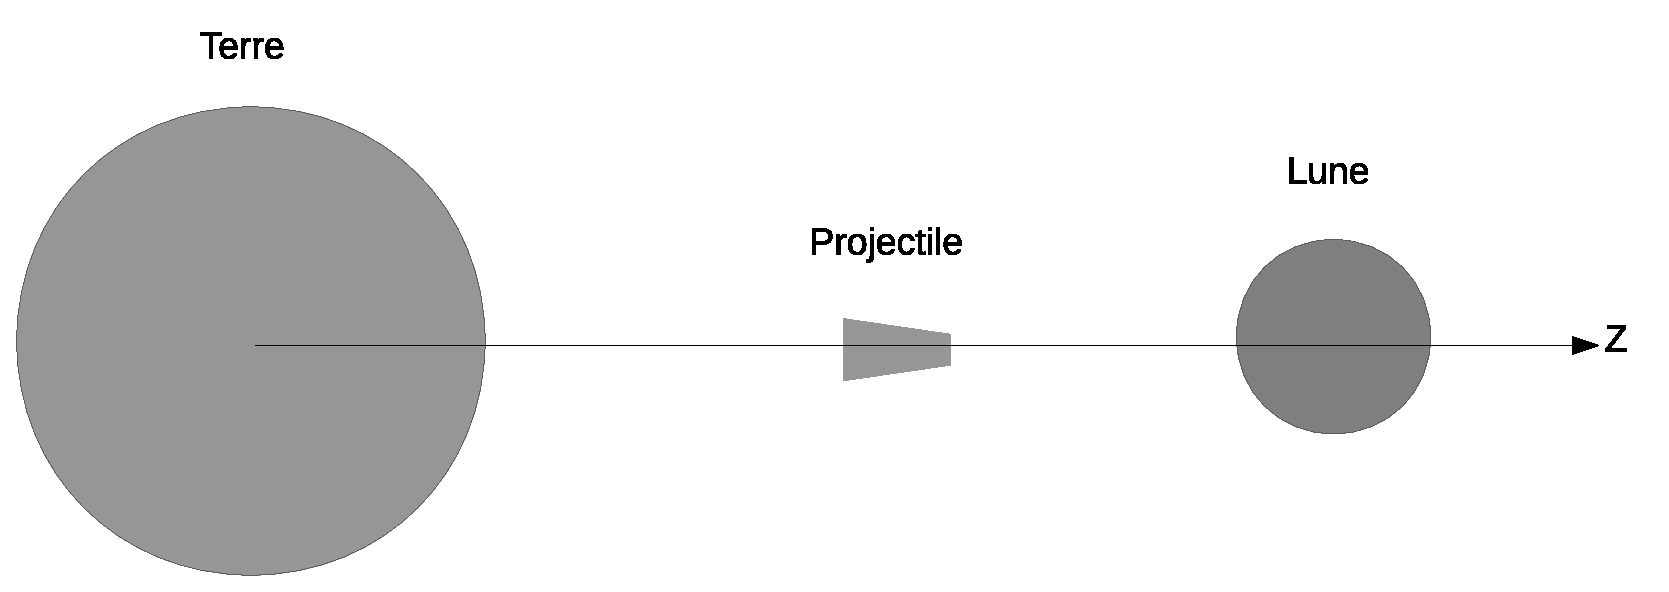
\includegraphics[width=.8\linewidth]{schema/schema.eps}
	\caption{Schéma de l'expérience}
	\label{fig:schema}
\end{figure}

\section{Solutions analytiques}
\subsubsection*{Question a}
Il est demandé d'établir une équation différentielle régissant notre problème.
Après quelques calculs qui seront décrit après l'équation, le résultat final est le suivant.
\begin{equation}
    \frac{d}{dt}
    \begin{pmatrix}
        z \\
        \dot{z}
    \end{pmatrix}
    =
    \begin{pmatrix}
    \dot{z} \\
    G\cdot\frac{m_L}{(z_L - z)^2} - G\cdot\frac{m_T}{z^2} - \frac{\rho_0}{m}\cdot e^{-\frac{z-z_0}{\lambda}}\cdot S\cdot C_x\cdot \frac{\dot{z}^2}{2}
    \end{pmatrix}
    \label{eq:sol}
\end{equation}

Cette solution nous permet donc de décrire la trajectoire du projectile, dans son périple entre la Terre et la Lune.
Cette solution comprend l'attraction de la Terre et de la Lune sur l'objet.
De plus, elle comprend une force de frottement visqueuse, qui ralentit le projectile lors de son passage dans l'atmosphère.\\

\subsubsection*{Question b}
Il est demandé de trouver le point d'équilibre de l'objet, s'il était statique.
Pour obtenir la solution, nous avons simplement égalisé les forces gravitationnelles appliquées sur le projectile, et isolé $z$.
Avec les valeurs fournies par le professeur, nous sommes arrivés au résultat suivant.

\begin{equation}
    z_E = \SI{3.460d8}{\meter}
    \label{val:zE}
\end{equation}

\subsubsection*{Question c}
Il nous est demandé de trouver, en négligeant l'atmosphère terrestre, la vitesse initiale qu'il faudrait pour que le projectile s'arrête sur le point d'équilibre.
Pour obtenir ce résultat, nous avons utilisé la conservation de l'énergie mécanique.
Nous avons donc considéré l'énergie mécanique du projectile lorsqu'il se trouve sur Terre, et lorsqu'il atteint le point d'équilibre.
Sur Terre, juste après le décollage, l'énergie du projectile se découpe en trois parties :
les potentiels gravitationnels de la Terre et de la Lune, et l'énergie cinétique du projectile.
Au point d'équilibre, il ne reste plus que les potentiels gravitationnels, car l'objet est à l'arrêt.
Ainsi, en isolant la vitesse, en utilisant les données du rapport et la position $z_E$ trouvée précédemment, nous sommes arrivés à ce résultat.

\begin{equation}
    v_0 = \SI{1.107d4}{\meter\per\second}
    \label{val:v0}
\end{equation}


\section{Résultats des simulations et réponses aux questions}
La deuxième partie de ce rapport se concentre sur l'implémentation numérique de ce problème afin de répondre aux questions posées.
À l'aide d'un schéma d'Euler, nous avons résolu numériquement l'équation différentielle et simulé, avec plusieurs pas de temps différents, notre problème.

\subsection{Question A - Simulation sans atmosphère}
Dans un premier temps, le système est simulé sur une durée de 24 heures en négligeant les effets de l'atmosphère.

\begin{figure}[h]
	\centering
    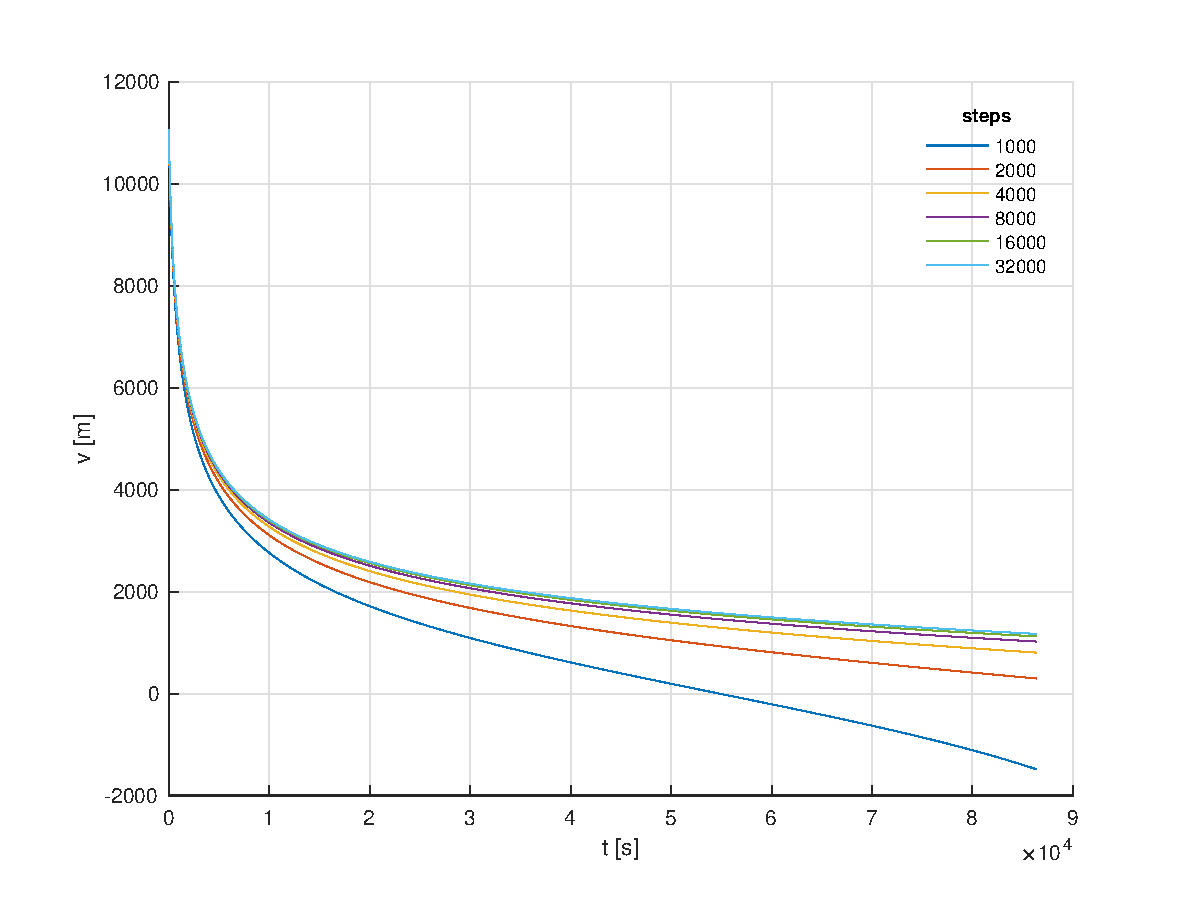
\includegraphics[width=0.53\textwidth]{graphs/vA.eps}
    \caption{Vitesse en fonction du temps}
    \label{fig:A-vt}
\end{figure}

On constate sur la figure \ref{fig:A-vt} que la vitesse diminue fortement au début de la simulation, en réponse à l'attraction terrestre, jusqu'à atteindre \SI{3500}{\meter\per\second} au bout de 3 heures, puis diminue beaucoup plus lentement après que le projectile se soit suffisamment éloigné de la Terre.\\

\begin{figure}[h]
	\centering
	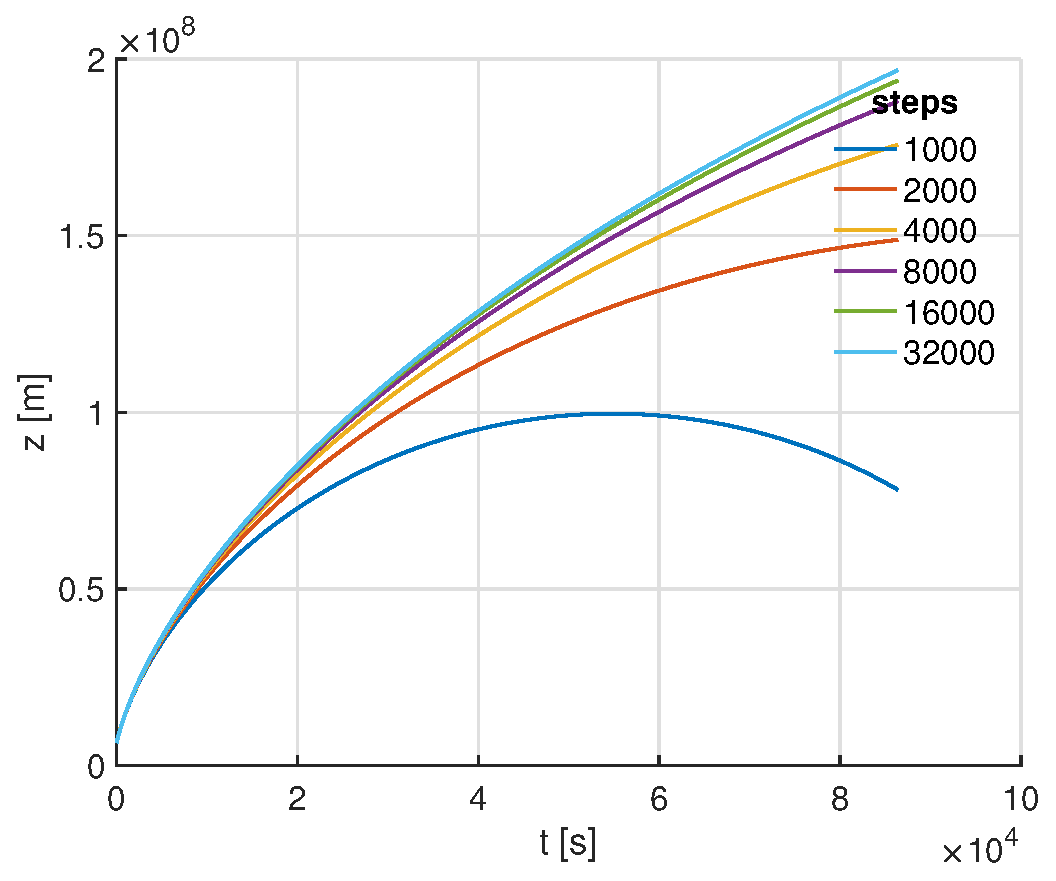
\includegraphics[width=0.53\textwidth]{graphs/zA.eps}
	\caption{Position en fonction du temps}
	\label{fig:A-zt}
\end{figure}

La figure \ref{fig:A-zt} montre que l'intégration par la méthode d'Euler est susceptible à de fortes imprécisions en-dessous d'un certain nombre de pas ;
en effet, dans la simulation avec nsteps=1000, la distance au point de départ diminue après 15 heures de vol, alors qu'elle continue d'augmenter dans les simulations avec un pas de temps plus petit.
On constate par ailleurs que le projectile parcourt une distance de \SI{200000}{\kilo\meter} en 24 heures.\\

\begin{figure}[h]
	\centering
	\begin{subfigure}[b]{0.45\textwidth}
		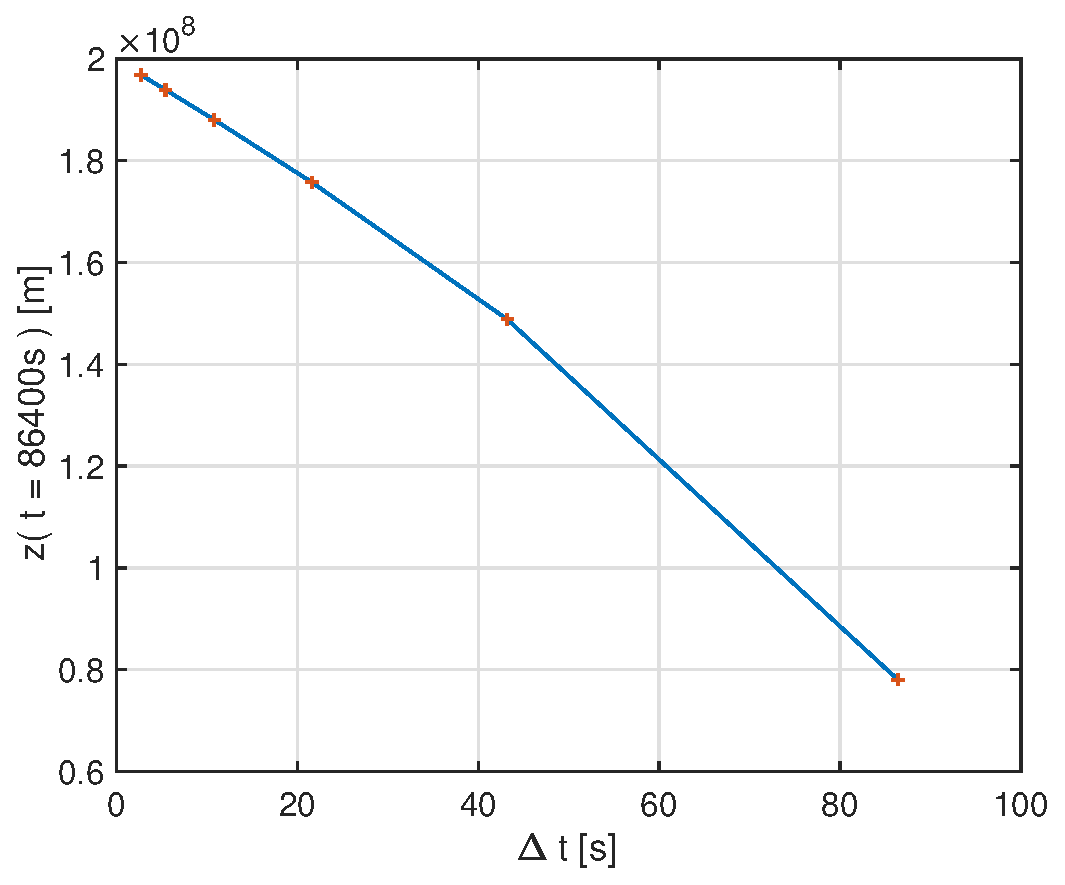
\includegraphics[width=\textwidth]{graphs/zConvA.eps}
		\caption{Graphique de convergence de la position}
		\label{fig:A-zConv}
	\end{subfigure}
	~
	\begin{subfigure}[b]{0.45\textwidth}
		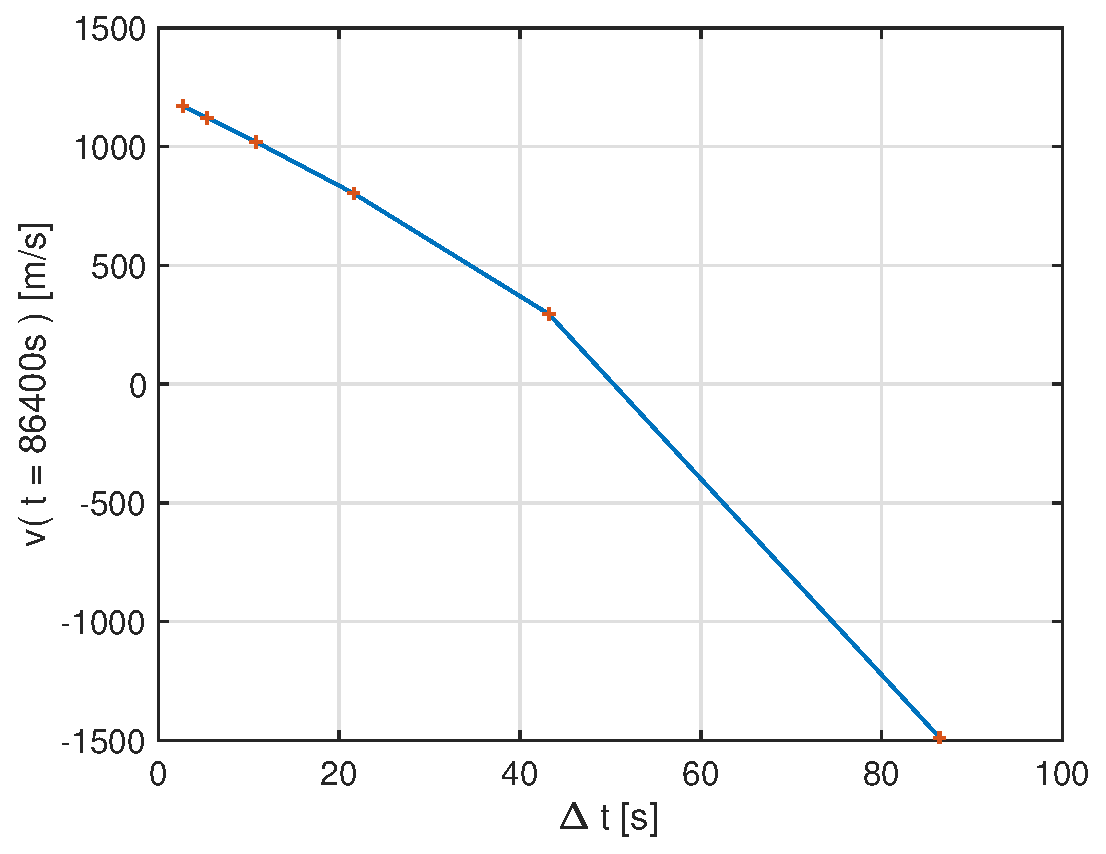
\includegraphics[width=\textwidth]{graphs/vConvA.eps}
		\caption{Graphique de convergence de la vitesse}
		\label{fig:A-vConv}
	\end{subfigure}
	\caption{Graphiques d'étude de convergence}
	\label{fig:A-conv}
\end{figure}

Les graphes de convergence de la position et de la vitesse (figure \ref{fig:A-conv}) montrent une convergence quasi-linéaire. 

\subsection{Question B - Simulation avec atmosphère}
Dans cette deuxième question, nous nous intéressons à la traversée de l'atmosphère, avec différents pas de temps.
Voici le résultat de ces simulations, durant les 10 premières secondes du décollage.\\

\begin{figure}[h]
	\centering
    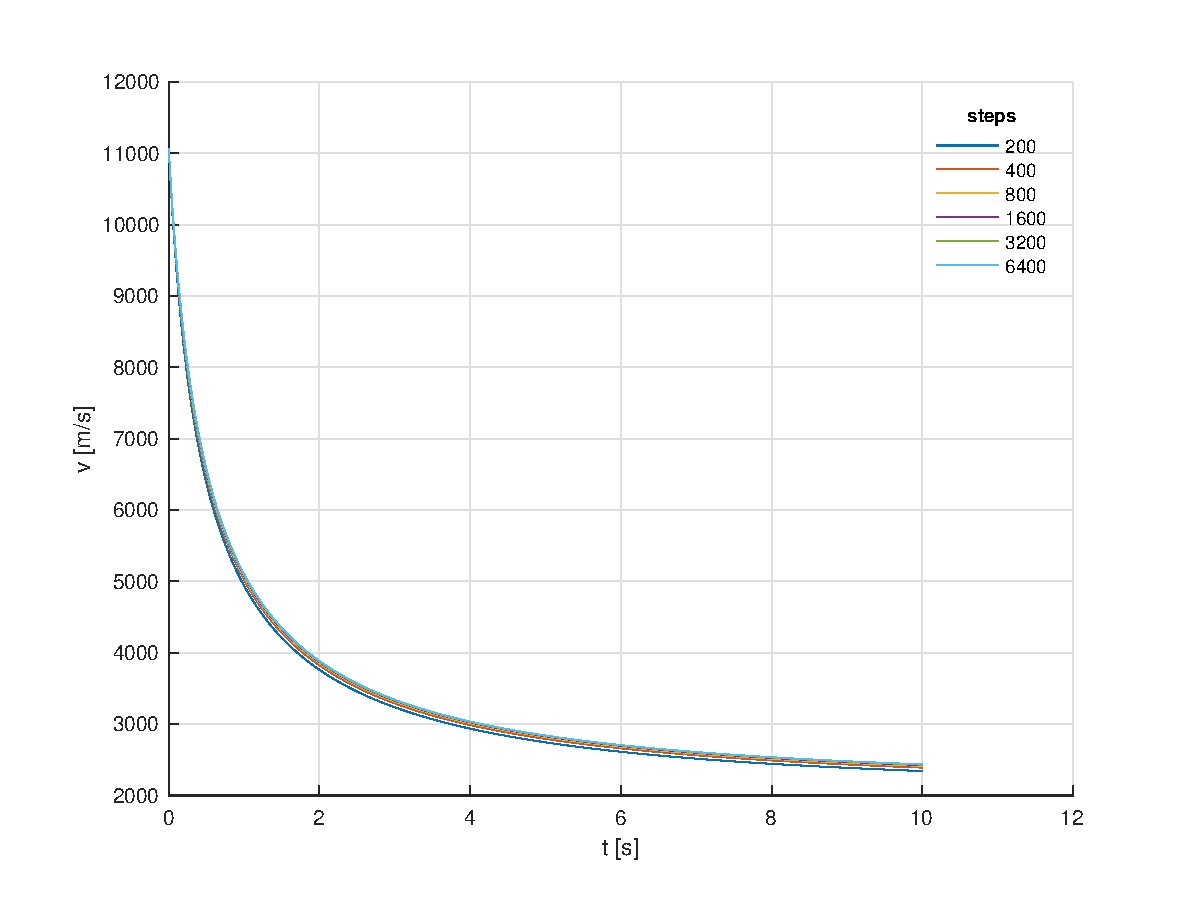
\includegraphics[width=0.53\textwidth]{graphs/vB.eps}
    \caption{Vitesse en fonction du temps}
    \label{fig:B-vt}
\end{figure}

Le projectile est très fortement ralenti par l'atmosphère, et cela se reflète sur la figure \ref{fig:B-vt}.
Les différences entre les courbes des différentes simulations sont minimes.
Au bout des 10 secondes de vol, le projectile a une vitesse de \SI{2500}{\meter\per\second}.
Cela s'explique par la vitesse au carré de l'équation \ref{eq:sol}, dans le terme aérodynamique.
En effet, la vitesse initiale $v0$ est très grande lors du décollage, ce qui implique que la force de traînée est très grande également.\\


\begin{figure}[h]
	\centering
	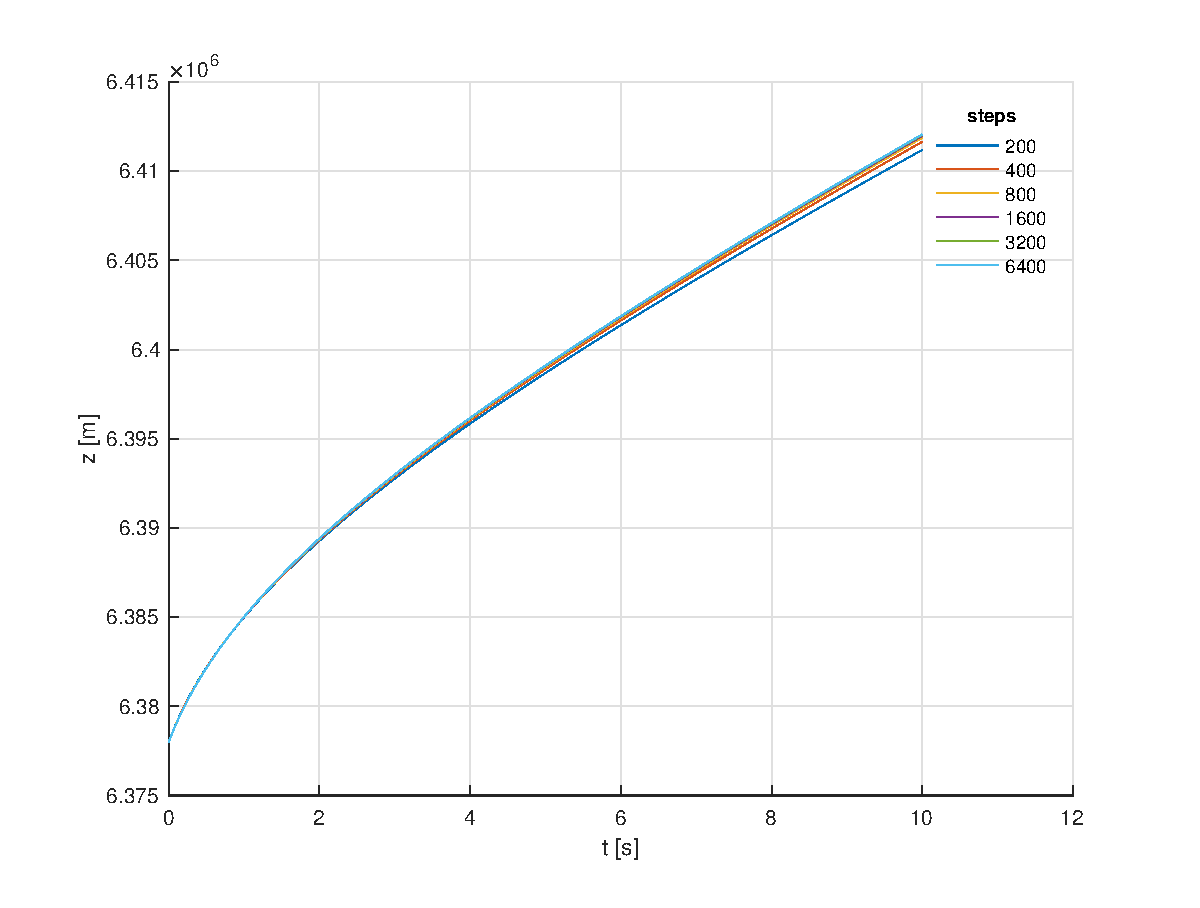
\includegraphics[width=0.53\textwidth]{graphs/zB.eps}
	\caption{Position en fonction du temps}
	\label{fig:B-zt}
\end{figure}

Concernant la tendance de l'accélération à tendre vers 0, elle provient du terme exponentiel de la force de traînée.
Ce terme provient du calcul de la densité de l'air, et il change de manière exponentielle lorsque la position change.
Les paramètres gravitationnels se retrouvent aussi dans ces graphiques, mais ils agissent sur le projectile de la même manière qu'à la question A, donc nous n'en parlerons pas plus ici.
Sur la figure \ref{fig:B-zt}, on observe que la position du projectile augmente drastiquement au début, mais ralentit rapidement son ascension en deux secondes, pour finalement augmenter de manière plus ou moins constante sur la fin.
Ainsi, au bout de 10 secondes, le projectile atteint une altitude d'environ \SI{40}{\kilo\meter} par rapport au sol terrestre.\\

\begin{figure}[h]
	\centering
	\begin{subfigure}[b]{0.45\textwidth}
		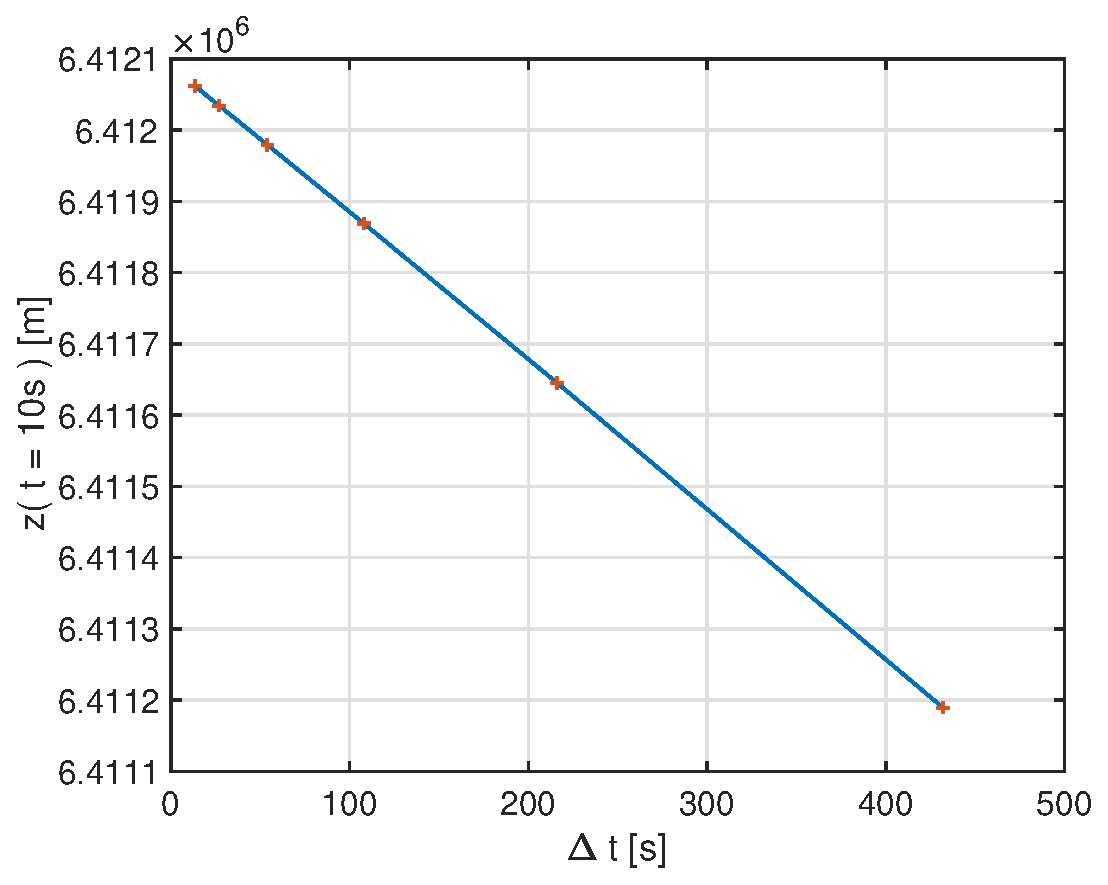
\includegraphics[width=\textwidth]{graphs/zConvB.eps}
		\caption{Graphique de convergence de la position}
		\label{fig:B-zConv}
	\end{subfigure}
	~
	\begin{subfigure}[b]{0.45\textwidth}
		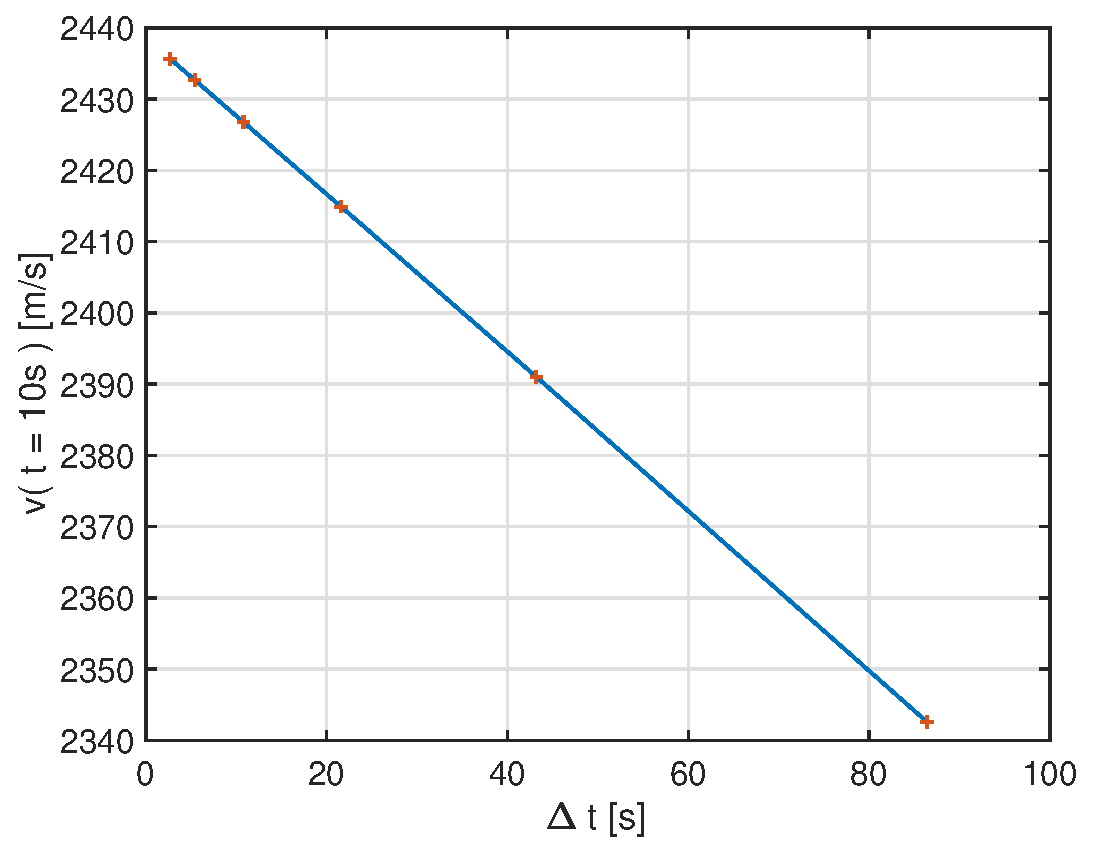
\includegraphics[width=\textwidth]{graphs/vConvB.eps}
		\caption{Graphique de convergence de la vitesse}
		\label{fig:B-vConv}
	\end{subfigure}
	\caption{Graphiques d'étude de convergence}
	\label{fig:B-conv}
\end{figure}

On constate sur la figure \ref{fig:B-conv} que la convergence de la position et de la vitesse finales sont linéaires.

\subsection{Question C - Bonus}
Pour des raisons de temps et techniques, cette question n'a pas pu être réalisée.
Nous en parlons plus en détail après.
Cependant, voici tout-de-même la manière qui aurait été mis en place si il avait été réalisé.
\begin{enumerate}
	\item À l'aide d'un script (shell par exemple), réaliser beaucoup de simulation en modifiant la vitesse pour chacune d'entre-elles, et enregistrer la position de chaques simulations.
	\item À l'aide de Matlab, réaliser un graph de la position en fonction de la vitesse choisie. Ainsi, il est possible d'estimer la vitesse que devrait avoir l'objet pour atteindre la lune.
	\item Après avoir drastiquement réduit le champ de recherche, refaire un script (shell) qui exécute avec des simulations avec des variations de vitesses plus faibles, ce qui augmente la précision de notre résultat.
	\item Finalement, trouver la vitesse idéale avec un graphique Matlab.
\end{enumerate}

Durant la tentative de réalisation de cette question, quelques obstacles se sont dressés.
Le principale problème renconté est le temps de simulation assez long.
Il était difficile de simuler beaucoup de cas, avec une bonne précision. 
En effet, pour effectuer cela, il aurait fallu considérer des millions de points sur des centaines de simulation, ce qui représente une quantité titanesque de calculs pour de simples ordinateurs domestiques.
Ensuite, en essayant de réduire légèrement la précision, afin d'obtenir une petite estimation, beaucoup de valeurs extrêmes sont apparues.
Cela a donc posé beaucoup de problèmes au niveau du graph, car ces points le rendaient illisible.

\section{Conclusion}
Le projectile de Jules Vernes s'apparente finalement à une fusée classique, bien que la méthode de propulsion soit différente.
Le succès de son voyage repose uniquement sur sa vitesse de départ.
Avec le v0 utilisé dans les questions A et B, le projectile arriverait donc à un point d'équilibre proche de la Lune. Il faudrait une vitesse initiale plus élevée pour atteindre la Lune elle-même.

Concernant la convergence, sans considérer la stabilité de notre schéma, il ressort de nos simulation qu'un petit pas de temps est important pour avoir une simulation précise.
Dans l'expérience A par exemple, le $\Delta$t choisi est dans la plupart des cas trop grand pour la simulation demandée, ce qui amène à des écarts conséquents entre les résultats des différentes simulations.
Le choix du $\Delta$t est donc primordial pour la réussite d'une simulation
Cela amène au problème suivant: les simulations sur une longue durée sont difficiles à réaliser sur un ordinateur domestique.
Pour avoir une précision raisonnable dans l'exercice B, on considérait jusqu'à plusieurs centaines de points par secondes, soit un $\Delta$t de l'ordre de la milliseconde pour les meilleurs cas.
Cette simulation a été possible pour un temps de simulation de 10 secondes.
L'exercice A, quant à lui, se concentre sur une simulation de 24 heures, soit 86'400 secondes.
Pour arriver à un $\Delta$t d'une dizaine de millisecondes, il faut déjà considérer plusieurs millions de points.
Et ce nombre augmente encore considérablement si la simulation est plus précise, ou si, comme dans l'exercice C, la simulation est plus longue.
Ainsi, il devient compliqué de réaliser des simulations sur une longue durée avec une bonne précision.
Il est donc indispensable d'adopter une meilleure stratégie pour la résolution des équations différentielles, afin d'augmenter la qualité des simulations, sans augmenter de manière démesurée le temps de calcul.


%  à partir de là, on se trouve dans les annexes
\appendix
\section*{Annexes}
\section{Cheminement analytique de l'équation différentielle}
Dans cette annexe, il sera décrit le cheminement pour arriver à l'équation \ref{eq:sol}.
Dans un premier temps, il faut considérer les forces appliquées sur le projectile.
Elles sont au nombre de 3:
\begin{itemize}
	\item La force gravitationnelle de la Terre: $\vec{F_T} = -G\frac{m_T m}{z^2}\vec{e_z}$ \cite{ref:ansermet}
	\item La force gravitationnelle de la Lune: $\vec{F_L} = G\frac{m m_L }{(z_L-z)^2}\vec{e_z}$
	\item La force de frottement visqueuse: $\vec{f} = - \rho S C_x \frac{v^2}{2}\vec{e_z}$ où $\rho (z) = \rho_0 e^{-\frac{z-z_0}{\lambda}}$
\end{itemize}

Ensuite, il faut considérer un bilan des forces.
\begin{equation}
	\text{Newton II: }\Sigma\vec{F}^{ext} = m\vec{a} \Leftrightarrow \vec{F_T} + \vec{F_L} + \vec{f} = m\vec{a}
\end{equation}

Projection sur l'axe dirigé par $\vec{e_z}$:
\begin{equation}
	-G\frac{m_T m}{z^2} + G\frac{m m_L }{(z_L-z)^2} - \rho S C_x \frac{v^2}{2} = m\ddot{z}
\end{equation}

Et en divisant par $m$, ainsi qu'en exprimant sous forme vectorielle cette équation, on obtient l'équation voulue \ref{eq:sol}.

\section{Cheminement vers la position d'équilibre}
Il suffit d'équilibrer les normes des deux forces gravitationnelles s'appliquant sur l'objet.
\begin{equation}
	F_T = F_L
\end{equation}
Et en réalisant l'application numérique, le résultat est bien la valeur \ref{val:zE}.


\section{Cheminement vers la vitesse initiale}
Pour arriver au résultat, il faut considérer l'énergie de l'objet.
le résultat découle de la conservation de l'énergie mécanique.
Il faut donc considérer deux moments dans la simulation: Le moment initial, et le moment où l'objet a atteint le point d'équilibre.
Dans un premier temps, considérer les potentiels suivants:
\begin{itemize}
	\item Potentiel gravitationnel de la terre en z: $E_{P,T} = -G\frac{m_T m}{z}$
	\item Potentiel gravitationnel de la lune en z: $E_{P,L} = -G\frac{m m_L}{z}$
	\item Energie cinétique à vitesse v: $E_C = \frac{1}{2}mv^2$
\end{itemize}

En considérant donc les deux moments de la simulation et la conservation de l'énergie mécanique:
\begin{equation}
	-G\frac{m_T m}{z_0} - G\frac{m m_L}{z_L - z_0} + \frac{1}{2}mv_0^2 = -G\frac{m_T m}{z_E} - G\frac{m m_L}{z_L - z_E}
\end{equation}

Et en isolant $v_0$, on obtient:
\begin{equation}
v_0 = \sqrt{-2G\frac{m_T}{z_E} - 2G\frac{m_L}{z_L - z_E} + 2G\frac{m m_L}{z_L - z_0} + 2G\frac{m_T m}{z_0}}
\end{equation}

Et avec l'application numérique: $v_0 = \SI{11.065}{\kilo\meter\per\second}$


% Description de la bibliographie
\begin{thebibliography}{99}

\bibitem{ref:ansermet}
	Jean-Philippe Ansermet,
	\textit{Traité de Physique: Mécanique},
	Presses Polytechniques et universitaires romandes, EPFL,
	2ème édition,
	p. 112,
	2015.


\end{thebibliography}

\end{document}